\documentclass{standalone}
\usepackage{circuitikz}
\usepackage{amsmath, amssymb}
\usepackage{siunitx}
\begin{document}
	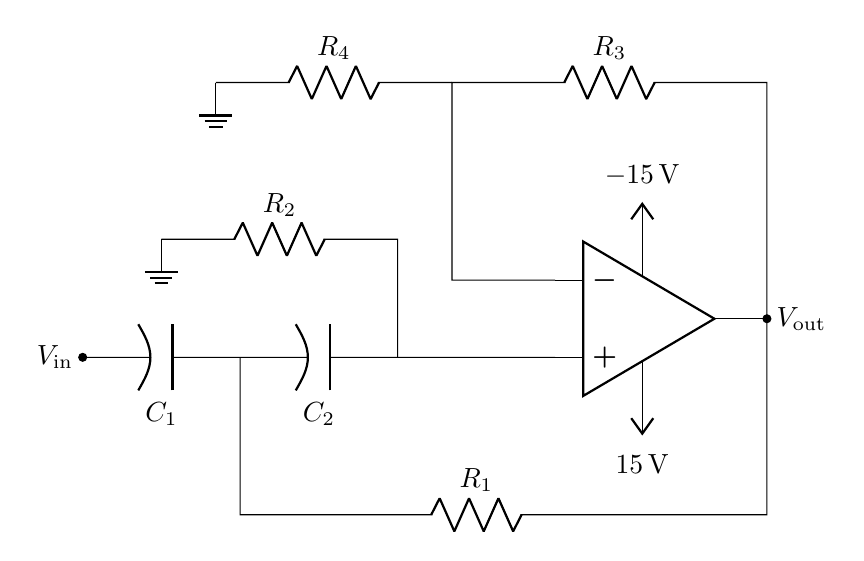
\begin{tikzpicture}
		\draw (0,0) node [op amp] (op) {};
		\draw (op.+) -- ++(-2, 0) to[pC, l=$ C_{2} $, invert] ++(-2,0) to[pC, l=$ C_{1} $, invert]
		++(-2,0) node(in) {};
		\draw (op.+) ++ (-2,0) -- ++(0,1.5) to[R, a=$ R_{2} $] ++(-3,0) node[ground] {};
		\draw (op.up) -- ++(0,0.5) node[vcc]{\SI{-15}{\volt}};
		\draw (op.down) -- ++(0,-0.5) node[vee]{\SI{15}{\volt}};
		\draw (op.+) ++ (-4, 0) -- ++(0, -2) to[R, l=$ R_{1} $] ++(6,0) 
		-| (1.5,0);
		\draw (op.out) -- (1.5,0);
		\draw (1.5,0) -- ++(0,3) to[R, a=$ R_{3} $] ++ (-4,0) |- (op.-);
		\draw (-2.5, 3) to[R, a=$ R_{4} $] ++ (-3,0) node[ground] {};
		\filldraw (in) circle [radius=0.05] node[left] {$ V_{\rm in} $};
		\filldraw (1.5,0) circle [radius=0.05] node[right] {$ V_{\rm out} $};
	\end{tikzpicture}
\end{document}